\begin{frame}{Kmeans: limitations}
\begin{itemize}
\item it can get stuck into bad local minima
\begin{itemize}
\item OPTIONAL: run the algorithm many times and choose the most recurrent solution
\end{itemize}
\item can only be employed in spaces where the mean operation is defined
\item due to its cost function, it can only cope with compact ball-shaped clusters
\begin{figure}
\begin{tabular}{cc}
\small{GT} & \small{Result}\\
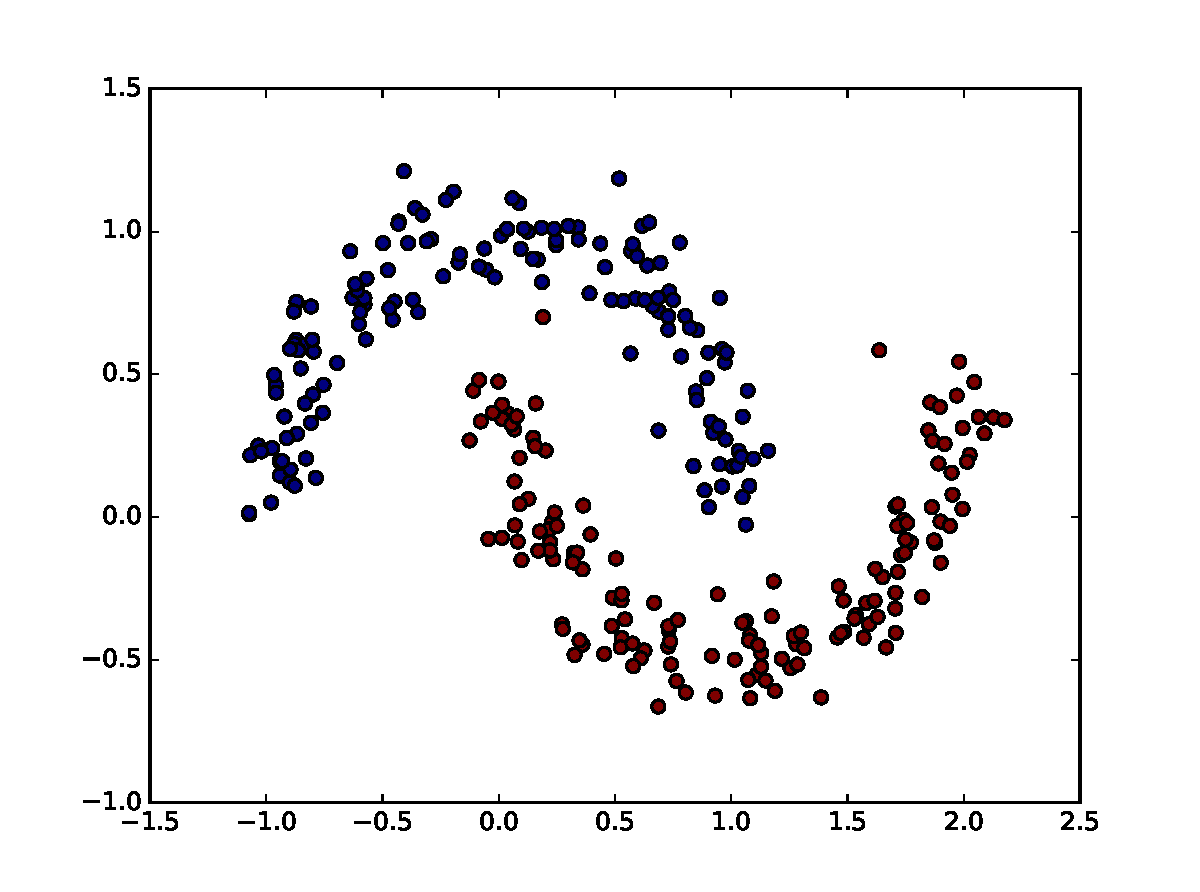
\includegraphics[width=0.35\textwidth]{img/kmeans/tm_gt.pdf}&
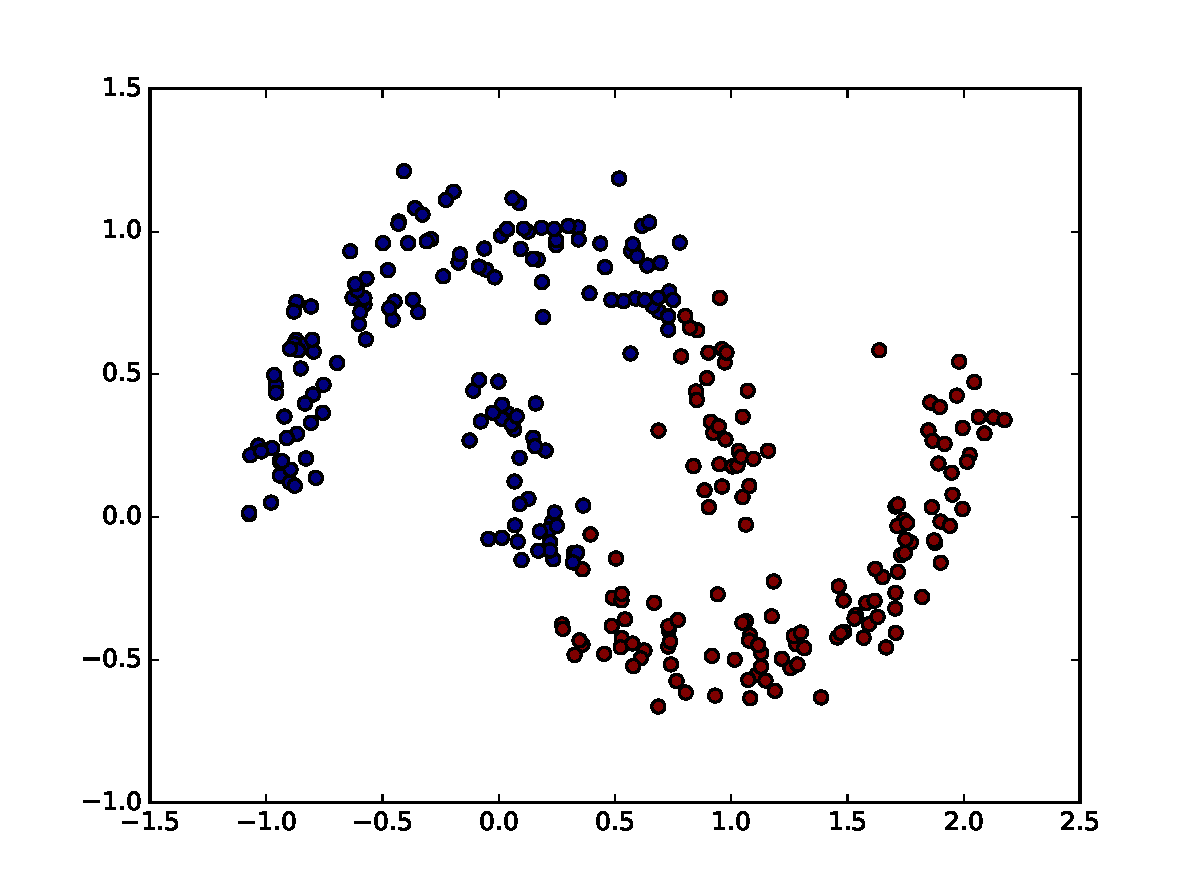
\includegraphics[width=0.35\textwidth]{img/kmeans/tm_fail.pdf}
\end{tabular}
\end{figure}
\end{itemize}
\end{frame}